
%: ----------------------- introduction file header -----------------------
\chapter{Introduction}

%\begin{flushright}
%I am just now beginning to discover the difficulty 
%\linebreak
%of expressing one's ideas on paper. As long as it 
%\linebreak
%consists solely of description it is pretty easy, but  
%\linebreak
%where reasoning comes into play, to make a proper
%\linebreak
%connection, a clearness \& a moderate fluency, is to me,   
%\linebreak
%as i have said, a difficulty of which i had no idea.
%\linebreak
%C. Darwin
%\end{flushright}
\ifpdf
    \graphicspath{{1_introduction/figures/PNG/}{1_introduction/figures/PDF/}{1_introduction/figures/}}
\else
    \graphicspath{{1_introduction/figures/EPS/}{1_introduction/figures/}}
\fi

In this PhD thesis, new Evolutionary Algorithm (EA) variants for solving large-scale design-optimization problems at reasonable computing cost are proposed, programmed and validated. This is extremely useful when handling large-scale industrial optimization problems, such as those in the fields of thermal and hydraulic turbomachines. The developed EA variants, enhanced with the proposed add-on features, must be able to produce high quality designs, at acceptable (according to the industrial standards) turn-around time. The latter is, in fact, necessary for EAs to become routinely used design-optimization tools in industrial environment, where the search method has to cope with a usually great number of design variables and computationally expensive evaluation codes.
 
A clear understanding of the reasons causing the drop in EA’s efficiency when used to solve industrial problems, particularly large-scale ones, is necessary before proceeding to the presentation of the proposed remedies. In this thesis, the problems under consideration are usually referred to as ``ill-posed’’. They are dealing with anisotropic (section \ref{IllCon}), non-separable (section \ref{Nonsep}) objective functions and have a great number N of design or optimization variables. The solution to an optimization problem  with a non-separable objective function, as opposed to a separable one, cannot be obtained by solving N distinct optimization problems, one for each design variable, since the optimal value of each one of them depends on the chosen values of the rest. In terms of N, this leads to superlinear increase in computational cost, in contrast to the linear increase expected in separable problems. It is evident that, for this type of problems, particularly if N is quite high, strong retardation in EAs convergence is expected. Note that the majority of industrial-scale problems are non-separable with a great number of unknowns.
 
The first way proposed in this thesis for reducing the optimization turn-around time relies on the replacement (during the EA-based search) of the standard shape parameterization techniques, which introduces a great number of design variables, by resorting to a number of available satisfactory designs.  In fact, this thesis proposes and evaluates a way to use the information residing into a small number of archived designs, made available from similar successful projects worked out in the past. This leads to optimization problems with much less unknowns which can be solved using EAs at noticeably lower computational cost. The new optimization variables are the coefficients introduced for merging the existing designs, in order to create new ones. The proposed method combines ``ideas'' from the theory of Knowledge-Based Systems (KBS) with EAs, giving rise to a fast design method, which will be referred to as Knowledge-Based Design (KBD). Though the proposed KBD method does not explicitly take care of the non-separability of the objective function with respect to the design variables, it is important that the number of optimization variables is greatly reduced. So, even without explicitly coping with the non-separability property, the gain in CPU cost is noticeable.
 
The second method proposed  herein makes use of the Principal Component Analysis (PCA) of promising/top individuals, in each generation of the EA, in order to identify directions in the design space which, if used to redefine the optimization variables, would result in ``better-posed'' optimization problems.  The redefinition of the optimization variables comes out from the alignment of each design vector with the so-called principal directions, computed by the PCA.  The evolution operators are applied to the transformed optimization variables and, for reasons to be explained as the text develops, an efficient search mechanism results, even without dimensionality reduction. 
 
Both the KBD method and the new way to apply the evolution operators driven by the PCA analysis of the current most promising solutions (such as the current front of non-dominated solutions in multi-objective optimization problems) can be used within either an EA or a Metamodel-Assisted EA (MAEA). In MAEAs, the costly problem-specific evaluation tool (herein, a Computational Fluid Dynamics or CFD code) is replaced by low--cost surrogate evaluation models or metamodels (trained artificial neural networks, ANNs, polynomial regression methods, etc.). In each generation, the CFD code is used to ``exactly'' evaluate a few of the most promising population members, as pointed by the metamodel(s).  
 
Regarding MAEAs, another way to further enhance their efficiency is by using the same PCA of the current promising solutions in order to associate each design variable (or design space coordinate) with a degree of importance. It will be shown that MAEAs may benefit a lot from the importance-based ranking of the design space coordinates, in order to overcome a well-known problem caused by the so-called curse of dimensionality. This problem is related to the fact that, for the ANNs used to approximate the fitness or cost of a new individual, any increase in the number of their sensory units calls for more training patterns and increased training cost.  Since the training patterns are selected among the previously evaluated individuals during the EA, the need for more training patterns means that the use of metamodels must be delayed. If, on top of this, each training is more costly, the gain from employing metamodels in lieu of the CFD code is expected to be lower or may even vanish. The proposed method is based on the selective truncation of the ANN entries, by maintaining only the most important design variables according to the results of PCA. It will be shown that, in real-world applications, the gain is important.   

The aforementioned methods are, firstly, validated in cases ranging from  some low-cost mathematical optimization benchmarks to 2D compressor cascade designs. Then, real-world problems such as the design of industrial 3D hydraulic turbines and the redesign of the 3D annular compressor cascade with tip clearance installed at the Lab of Thermal Turbomachines of NTUA (LTT/NTUA) are examined. The mathematical benchmarks have low computational cost and allow the exhaustive investigation of methods by repeating the runs on the same case, using different seeds in the random number generator. By doing so, the conclusions reached are safe. The presented 2D cases allow the demonstration of the proposed methods in simple aerodynamic cases. In the field of hydraulic turbomachines, two types of hydraulic turbines, a Francis and a new type named Hydromatrix$\circledR$, are used to validate the performance of the aforementioned methods in large-scale industrial applications. A number of performance metrics are introduced and, depending on the case,  are combined to form the necessary objectives and constraints. In the hydraulic turbomachinery design problems, more than one operating points are considered, leading to increased cost per evaluation. This makes the reduction in the number of evaluations required to reach the optimal solution(s) absolutely necessary.  In the field of thermal turbomachines, the blade airfoil of the 3D compressor cascade installed at LTT/NTUA is optimized for minimum total pressure losses.     


This PhD thesis is based on EAs developed during a number of previous PhDs \cite{phd_Giotis,phd_Karakasis,phd_Kampolis,phd_Vera} performed at the Parallel CFD \& Optimization Unit of LTT/NTUA (PCOpt/NTUA). These PhD theses created the algorithmic basis or software platform,  which the newly proposed methods are built upon. This EA-based optimization platform, known as EASY (Evolutionary Algorithm SYstem \cite{EASYsite}) includes the basic EA, optionally enhanced by parallel search (Parallel EAs or PEAs), the use of ANNs as metamodels (MAEAs) and hierarchical optimization schemes (Hierarchical EAs or HEAs). EASY provided fertile ground for the development of all methods proposed by this PhD thesis.                       
 
%An overview of the use of optimization methods for fluid dynamic problems, a review on the previews works by PCOpt this thesis has build upon and the thesis structure follow.
 
\section{CFD-Based Optimization}

In this section, an overview of CFD-based optimization methods is presented. CFD-based optimization methods enjoy great interest from both academia and industry since the performance and, therefore, the price of products (ranging from cars and aircrafts to thermal and hydraulic turbomachines etc.) depends heavily upon their aero/hydrodynamic performance. 

\begin{figure}[h!]
\begin{minipage}[b]{1\linewidth}
 \centering
 \resizebox*{!}{8 cm}{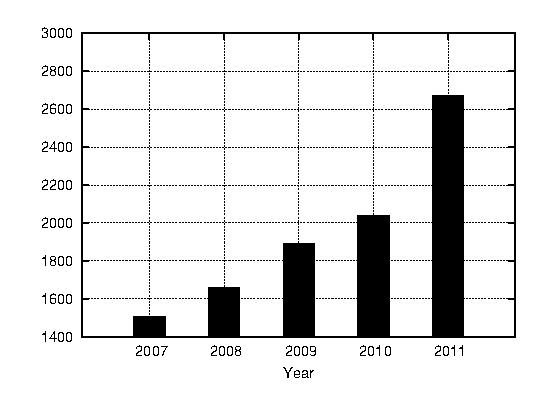
\includegraphics{OptimizationCFD.eps}}
\end{minipage}
\caption{Yearly number of publications on CFD-based optimization appearing in ScienceDirect.} 
\label{pubs.CFD}
\end{figure}

In order to demonstrate the increasing interest of the scientific community in CFD-based optimization, an internet-based literature survey was carried out using the search tool ``ScienceDirect'' (http://www.sciencedirect.com/). The search lemma was (Optimization $AND$ CFD) $OR$ (Optimization $AND$ Computational Fluid Dynamics).  This is obviously a non-exhaustive search; it is though good enough to show trends.  The steadily growing number of publications in the last five years, shown in fig.\ \ref{pubs.CFD}, reveals the growing interest in performing CFD-based optimization. Therefore, it is expected that the upgrades proposed in this thesis must be of interest to a continuously growing in size community of scientists, not necessary restricted to those working in the field of turbomachines.     
 
A prerequisite for any shape optimization problem in fluid dynamics is the availability of a fast and reliable way to evaluate candidate solutions. This is achieved through the use of CFD (hence the term CFD-based optimization) methods that numerically solve the differential equations governing the fluid motion. Nowadays, thanks to the relatively cheap access to powerful computational means, the CFD tools have affordable CPU cost (depending on the case complexity) and, therefore, optimization methods based on them are flourishing. The strong dependence of the CFD-based optimizations on the computational resources becomes crucial in cases where a number of disciplines (ranging from structural analysis to manufacturing and economics, etc.) are used to evaluate the candidate solutions (multi-disciplinary optimization, MDO). The fact that the fluid dynamic, structural and economical objectives may be contradictory adds extra difficulty to the optimization procedure.           
 
An important part of any optimization project is the definition of the design variables. An optimization algorithm seeks the value set of the design variables which minimizes the user-defined cost function(s).  In CFD-based optimization, typical objectives are: maximization of lift,  minimization of drag,  maximization of efficiency, minimization of the deviation from given target (pressure, velocity, etc.) distributions, minimization of viscous or shock-induced losses or the cavitation index (in hydraulic turbomachines), etc. One (single-objective optimization, SOO) or combinations of them can be used. Design-optimization problems with more than one objectives (multi-objective optimization, MOO) can be solved by concatenating the objectives into a single one, after multiplying them with appropriate weights. The difficulty of choosing the most appropriate weight values and the failure of this approach in non-convex optimization problems are the main weaknesses of this approach.  An improved way to solve MOO problems is the use of dominance-based methods that rank the candidate solutions according to Pareto dominance \footnote{Solution $a$ dominates solution $b$ if and only if $a$ is equal to $b$ with respect to all objectives but one and better than $b$ at least for one of them.}. These methods compute a set of optimal solutions forming the so-called front of non-dominated solutions or Pareto front, where none of them is dominated by any other front member with respect to all objectives.  Therefore, the choice of the optimal solution to be adopted relies upon additional criteria set by the decision-maker.  The design-optimization problem can, also, be subject to a number of constraints. In shape optimization related to fluid mechanics, constraints are imposed to geometrical quantities (for instance, thickness constraints so as to come up with manufacturable designs), structural quantities such as the maximum stress or deflection and/or flow-related quantities such as the minimum flow turning or the cavitation index, in turbomachines.          

In general, CFD-based shape optimization methods can be classified in two categories, namely direct and inverse ones. Direct methods \cite{phd_Giotis,phd_Kampolis,phd:papadim,kn:Emm2002,kn:Emm2004} solve the optimization problem through a number of trials that involve the geometry generation, CFD-based flow predictions, the computation of the objective function and, if necessary, its gradient computation.  On the contrary, inverse methods (should not be confused with inverse design problem \footnote{Inverse design problems use the deviation of the current from a desirable flow variable distribution as cost function.} that can be solved by direct methods) \cite{chav:95,ded:95} begin from a set of desirable flow field characteristics (such as those related to the boundary layer) and solve the inverse problem to define the geometry. The major advantage of inverse methods is their low cost and the fact that they don't need a starting geometry. On the other hand, their most noticeable drawback is the inability to handle constrained optimization problems. The inverse methods developed by LTT/NTUA are based on the Le Foll method \cite{lefoll} which is an integral method using a two-parametric boundary layer velocity profile. This method was extended to accommodate compressibility \cite{pap69}, surface curvature effects on the turbulent boundary layer \cite{pap70} and boundary layer separation \cite{pap81} and was used for the design of both axial and radial turbomachines. Based on the above classification, this PhD thesis is dealing with direct design-optimization methods.  

Based on the way optimal solutions are sought, the optimization methods can be classified as deterministic and stochastic. In CFD-based optimization, deterministic methods were used first,  mainly due to their solid mathematical background and fast convergence, to locate optimal solutions with less trials. Deterministic methods require the computation of the gradient of the objective function with respect to the design variables. This limits the type of objective functions such a method might handle to those being differentiable. The cost of the gradient calculation might become prohibitive if access to the evaluation software source code is not granted and computationally expensive finite-difference schemes must be employed. On the other hand, in MOO problems, they have difficulties to compute fronts of non-dominated solutions with a single run and they risk of being trapped into local minima.        

In the deterministic or gradient-based optimization methods used in fluid dynamics, the most important part is the gradient computation. The use of finite differences, as mentioned above, is not suitable since it requires, at least, as many flow analyses as the design variables. The use of adjoint techniques can reduce this cost to that of a single-equivalent flow solution irrespective of the number of design variables. Due to the need of significant investment in person-months (mathematical development and programming) required for the development of the adjoint methods and software, these were not used in CFD-based optimization since mid $80's$ \cite{piron:84, kn:Jame88, kn:Jame94, kn:Jame95}.  The two variants of adjoint techniques, discrete and continuous, differ in the way the discretized adjoint equations are formed. The continuous adjoint method \cite{kn:Jame94, kn:Ander99,phd:papadim} processes the flow PDEs to derive the adjoint ones which are, then, discretized. On the other hand, in the discrete adjoint method, the adjoint equations result directly from the discretized flow equations, \cite{kn:Elliott96, anderson:99}. A more detailed presentation of adjoint methods used for fluid dynamic optimization can be found in \cite{phd:papadim}.        

On the other hand, stochastic optimization methods  do not suffer from the risk of getting trapped into local minima due to the probabilistic search they employ. The differentiability of the objective function is not required. An additional advantage of stochastic optimization methods, especially regarding industrial usage, is their ability to handle any problem, by merely accommodating the available evaluation software, without even having access to its source code. Their main drawback, though, is the need to evaluate a great number of candidate solutions before reaching the optimum. This may significantly increase the overall computational cost of the optimization procedure. This PhD thesis is dealing with stochastic optimization methods and, more precisely, EAs and aims at the reduction of computational cost. 

The use of EAs in CFD-based optimization was delayed until mid $90's$, mainly due to their high computational cost. The first relevant works \cite{kn:Quag95,per:95,kn:Gala96} presented automated EA-based procedures for aerodynamic design-optimization problems. Soon after, emphasis was laid on the reduction of the cost of the overall optimization procedure, mainly by adapting the available variable representations and evolution operators. This continued with their hybridization with deterministic methods. For instance, in \cite{kn:Mar97} and \cite{kn:Fost97}, an EA was used to spot a good starting solution for a deterministic optimization method. In \cite{dennis:99}, EAs were hybridized with Sequential Quadratic Programming (SQP) for constrained shape optimization problems. Furthermore,  the use of distributed EAs \cite{kn:Door1997,kn:SefrThes}, surrogate evaluation models \cite{kn:Ratl98,kn:Gio99,kn:Gian1999,kn:EBNK,phd_Kampolis}, hierarchical schemes \cite{kn:Eby1998,kn:Sef2000,knowles00mpaes_x41,desideri03,phd_Kampolis} and concurrent evaluations on a multiprocessor platform \cite{kn:LeeH96,phd_Giotis,phd_Vera} have been proposed. Nowadays, the appeal of CFD optimization using EAs for industrial-scale engineering problems is growing due to the availability of powerful computational resources. This PhD thesis is dealing with the use of EAs for solving industrial-scale design-optimization problems in the fields of thermal and hydraulic turbomachines in acceptable (for industry) turn-around time.   


\begin{figure}[h!]
\begin{minipage}[b]{1\linewidth}
 \centering
 \resizebox*{!}{8 cm}{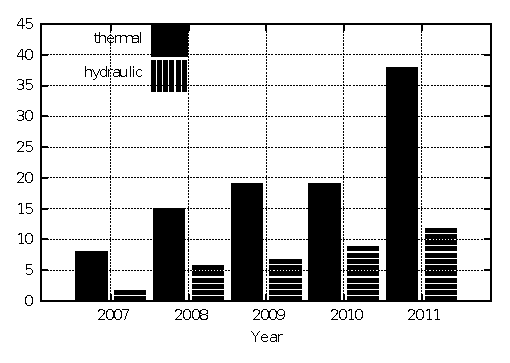
\includegraphics{hydrtherm_m.eps}}
\end{minipage}
\caption{Yearly number of recent publications which are relevant to the optimization of thermal and hydraulic turbomachines, in ScienceDirect.} 
\label{pubs.turbo}
\end{figure}
 

Regarding CFD-based optimization in the fields of thermal and hydraulic turbomachines, another internet-based literature survey was carried out, too. The search lemmata were: (a) optimization $AND$ thermal $AND$ turbomachines and (b) optimization $AND$ hydraulic $AND$ turbomachines. This survey reveals the steadily growing number of publications, in both turbomachinery areas, over the last five years, as shown in fig.\ \ref{pubs.turbo}. 

For instance, in the ASME 2011 Turbo Expo Conference, $24$ papers were about the development and applications of EA-based optimization in the field of thermal turbomachines; some of them are not CFD-based. Most of them are handling a small number of design variables, $(N\!\leq\!15)$, and only three \cite{Georg2011,Marcel2011,Kevin2011} solve high-dimensional problems $(N\!>\!30)$. In \cite{Georg2011}, the application of an axisymmetric endwall contour for compressors is investigated. An EA-based optimization of the outer casing and the corresponding blade tip airfoil section of a typical gas turbine high-pressure compressor stage, with a high number of design variables ($N\!=\!38$), is presented. In \cite{Marcel2011}, the high-dimensional ($N\!=\!210$) constrained MOO of a fan stage, using EAs enhanced by metamodels, is presented. In \cite{Kevin2011}, an EA-based axisymmetric multi-disciplinary optimization approach for compressors is  applied to the design of a three-stage booster with $N\!=\!53$ design variables. Even though the aforementioned papers use a great number of design variables, they typically start from an almost optimal design and, therefore, are able to significantly restrict the design space per design variable. For instance,  \cite{Marcel2011} starts from a ``pre-optimized'' design and in \cite{Georg2011} the search space of each design variable is of the order of the tip clearance magnitude (very small). Note that the KBD method proposed by this thesis may efficiently deal with both high-dimensional ($N\!>\!300$) problems with extended search space per variable.      

In the IAHR 2010 conference, $5$ paper on the optimization of hydraulic turbomachines were presented. Three of them,  \cite{Raimunda2010,Kyriacou2010,Popa2010} used EAs. In \cite{Popa2010}, the weekly operation of a multipurpose
hydroelectric development, including a pumped storage plant was optimized using an EA. In \cite{Raimunda2010}, an optimization problem with two design variables, concerning the design of an axial compressor cascade using a MAEA was presented.  In \cite{Kyriacou2010}, the author of this thesis presented the solution of an optimization problem with $336$ design variables, concerning the design of a Francis hydraulic turbine. 


Research on the CFD-based optimization in the fields of thermal and hydraulic turbomachines was carried out in the Laboratory of Thermal Turbomachines (LTT/NTUA) and the Laboratory of Hydraulic Machines (LHM/NTUA) of NTUA. 
Concerning thermal turbomachines, a number of papers regarding both deterministic and stochastic optimization methods reflect the performed research at LTT/NTUA. Most of them are related to the optimal design of components of thermal turbomachines, such as compressor cascades, using a variety of optimization methods.  An indicative subset of them is mentioned below. The coupling of stochastic optimization methods with computational intelligence is presented in \cite{LTT_2_018,LTT_2_020,LTT_2_023}. There, the use of artificial neural networks as metamodels, in order to assist  EAs incorporating costly evaluation tools such as CFD codes, are proposed. In \cite{LTT_2_026}, the use of metamodels trained  on both responses and gradients is proposed and used in the inverse design of a 3D peripheral cascade. In \cite{LTT_2_031}, the hierarchical distributed MAEA is used for the viscous loss minimization of a compressor cascade. In \cite{LTT_2_040}, an asynchronous EA is demonstrated on the  design of a 2D compressor cascade and in \cite{LTT_2_045} a grid-enabled asynchronous MAEA is applied to the optimization of a 3D annular compressor cascade. In \cite{LTT_2_032}, an adjoint-based optimization method is proposed for the total pressure losses minimization in turbomachinery cascades.  In \cite{LTT_2_049},  the computation of the exact Hessian matrix of the objective function measuring total pressure losses in turbomachinery cascades is presented for use along with Newton methods. Multi-level strategies that combine adjoint-based methods with MAEAs for turbomachines are described in \cite{LTT_3_092}.


Concerning the CFD-based optimization in the field of hydraulic turbomachines, the work done at LHM/NTUA is related to: a) the design of optimal components of hydraulic machines, such as runner blades, and b) the optimal design of complete hydroelectric power plants and energy storage plants in combination with other forms of renewable energy generation sources, such as wind energy. Indicatively, in \cite{Anagno2}, an EA is used to improve the design of a ``Tesla-type'' valve for micropumps. In \cite{Anagno4}, the fast Lagrangian approach is incorporated into an EA to design an optimal Turgo turbine. The optimal sizing of a run-of-river small hydroelectric power plant utilizing an EA is described in \cite{Anagno3}. In \cite{Anagno5,Anagno6}, the optimization of pumped-storage systems for wind power plants is presented.

   

\section{EAs: Previous work at PCOpt/NTUA} % section headings are printed smaller than chapter names
\label{PRW}
An overview of previous PhD theses on EAs which were carried out by PCOpt/NTUA research group follows. 

Giotis' thesis \cite{phd_Giotis}, developed a generalized EA able to combine components of the two most widely used evolutionary optimization methods, namely Genetic Algorithms (GAs) and Evolutionary Strategies (ESs). In the same thesis or the corresponding papers \cite{kn:Emm2002,LTT_2_018,LTT_2_023}, the use of artificial neural networks as local metamodels, trained on previously evaluated candidate solutions, was proposed in order to reduce the computational burden. To reduce the wall clock time of the optimization, parallel evaluations of candidate solutions on a number of available processors, via the PVM protocol were used. The EASY optimization platform this thesis relies upon originated from Giotis thesis \cite{phd_Giotis}.   

Karakasis' thesis \cite{phd_Karakasis}, further improved the EA efficiency by focusing on the optimal use of metamodels in MOO problems. One of the most important outcomes of this thesis was that the MAEA became equally efficient in both SOO and MOO, by overcoming problems related to: (a) the fact that, in MOO, the previously computed individuals, by the EA are spread along a front in the design space rather than clustered around the sought optimal solution and (b) the presence of outliers that require special treatment. Distributed EAs (DEAs) were programmed and validated, in order to increase the parallel efficiency of EAs and avoid stagnation during the early generations. Furthermore, the notion of Hierarchical EAs (HEAs) was introduced and this  was later refined in \cite{phd_Kampolis}.    In \cite{phd_Karakasis}, the use of a DEA on each level of the HEA associated with a different evaluation model was proposed.

In Kampolis' thesis \cite{phd_Kampolis}, the HEAs were upgraded by introducing hierarchical schemes other than those based on the combined use of low- and high-fidelity evaluation software. The latter made use of different parameterization schemes (coarse and fine) or different search methods allowing, thus, the combination of EAs with deterministic optimization methods. Finally, new artificial neural networks trained on both the objective functions values and their gradient were proposed, see also \cite{LTT_2_026}.          

Asouti's thesis \cite{phd_Vera}, proposed a different way to increase the parallel efficiency of EAs or MAEAs. This was achieved by introducing the so-called Asynchronous EAs (AEAs) or Asynchronous MAEAs (AMAEAs). By utilizing a number of strongly interconnected demes, according to a newly proposed topology, the asynchronous variants may circumvent the ``end of generation" synchronization barrier and, thus, uninterruptibly use all the available processors.     The proposed AEAs and AMAEAs are appropriate for heterogeneous multi-processor platforms. 


Georgopoulou's thesis \cite{phd_Chara}, proposed the so-called Metamodel-Assisted Memetic Algorithm (MAMA). Memetic Algorithms (MAs) are hybrid
methods that combine stochastic and deterministic search methods. The proposed MAMA combines the advantages of both MAEAs and MAs.
 
In a sixth PhD \cite{phd_eugene}, Kontoleontos also used the EASY platform to optimize heat transfer systems, such as
geothermal power plants and ground source heat pump systems.
 
 
\section{Thesis Outline} % section headings are printed smaller than chapter names
A short overview of the chapters of this PhD thesis follows:

Chapter $2$ presents the pre-existing algorithmic basis of this PhD. This includes the generalized EA with its evolution operators, the MAEA and the HEA.

Chapter $3$ is concerned with the first innovative method proposed in this PhD thesis, namely the Knowledge-Based Design (KBD) one. In the first part of this chapter, a short overview of KBS is presented. Then, the proposed KBD method is described in detail and used to perform the design of a 2D compressor cascade, in order to demonstrate its merits.

Chapter $4$ is dealing with EAs and MAEAs suitable to solve ill-posed optimization problems. This chapter starts by describing the features of ill-posed optimization problems. Then, the drop in EA efficiency when used to solve ill-posed problems is investigated. An innovative way to find new directions in the design space that, if used to redefine the design variables, would result in a better-posed problem that can be solved using EAs and MAEAs at lower computational cost is proposed.  New evolution operators, the so-called PCA-driven ones, are devised, in order to recover the aforementioned EA efficiency drop. Furthermore, the use of the importance information, resulting from the PCA is used to enhance metamodel's efficiency. Finally, the gain achieved using the proposed methods is quantified through the study of a 2D compressor cascade design-optimization case.

In Chapter $5$, the methods proposed in Chapters 3 and 4 are used to solve large-scale industrial problems in the field of hydraulic turbomachines. The parameterization, grid generation and CFD tools used in this studies are presented. Quality metrics measuring each hydraulic turbine quality with respect to cavitation, blade loading and draft-tube coupling are introduced. Then, the optimization of a Francis turbine, in the context of a modernization/rehabilitation project, is used to demonstrate the merits of the KBD method, by comparing it with a conventional EA. Also, the optimization of a new type of hydraulic turbine, the so-called Hydromatrix$\circledR$, is carried out in order to demonstrate the gain expected from MAEAs using the proposed PCA-driven evolution operators.

Chapter $6$ is dedicated to the design-optimization of the compressor cascade installed at LTT/NTUA. This case is used to investigate the combined effects of the use of PCA-driven evolution operators and the PCA-assisted metamodels,  proposed in Chapter $4$.

Finally, Chapter $7$ summarizes the conclusions drawn in this PhD thesis.      

%: ----------------------- HELP: references
% References can be links to figures, tables, sections, or references.
% For figures, tables, and text you define the target of the link with \label{XYZ}. Then you call cross-link with the command \ref{XYZ}, as above
% Citations are bound in a very similar way with \cite{XYZ}. You store your references in a BibTex file with a programme like BibDesk.


%%%%%%%% template for figures
%see fig \ref{A common glucose polymers}
%\figuremacro{EAvsPCA_zdt3}{A common glucose polymers}{The figure shows starch granules in potato cells, %taken from \href{http://molecularexpressions.com/micro/gallery/burgersnfries/burgersnfries4.html}{Molecular %Expressions}.}

%%: ----------------------- HELP: adding figures with macros
%% This template provides a very convenient way to add figures with minimal code.
%% \figuremacro{1}{2}{3}{4} calls up a series of commands formating your image.
%% 1 = name of the file without extension; PNG, JPEG is ok; GIF doesn't work
%% 2 = title of the figure AND the name of the label for cross-linking
%% 3 = caption text for the figure

%%: ----------------------- HELP: www links
%% You can also see above how, www links are placed
%% \href{http://www.something.net}{link text}

%\figuremacroW{EAvsPCA_zdt3}{Title}{Caption}{0.8}
%% variation of the above macro with a width setting
%% \figuremacroW{1}{2}{3}{4}
%% 1-3 as above
%% There you go. You already know the most important things.



